\chapter{Conclusions}
\label{chap:conclusions}


The main goal of this thesis was to develop a 3D MOC solver capable of accurately and efficiently simulating LWR models for a fixed but reasonable choice of cross-sections. This goal was motivated by the desire to develop methods which can explicitly handle axial as well as radial variation within PWR reactor cores. The following summarizes the key accomplishments demonstrated by this thesis to meet this challenge:

\begin{itemize}
	
	\item \textbf{The implementation of an efficient 3D MOC solver.} A 3D MOC solver was implemented in OpenMOC which is capable of efficiently solving the MOC equations using an efficient track laydown, on-the-fly ray tracing, and spatial domain decomposition. In addition, an efficient linear source solver was added, allowing for accurate solutions with relatively coarse mesh.
	
	\item \textbf{Theoretical and practical evaluation of source iteration convergence.} The convergence of transport codes using source iteration (such as MOC) with transport-corrected cross-sections has plagued researchers in the past. In this thesis, a robust theoretical framework is introduced to understand convergence characteristics. The diagonal stabilization scheme was presented which alleviates the convergence issues.
	
	\item \textbf{3D MOC parameter refinement studies.} Since previous 3D MOC solvers have not been capable of solving large PWR problems, parameter refinement studies have not been fully explored. In this thesis, the sensitivity of solution accuracy to each 3D MOC parameter is thoroughly explored.
	
	\item \textbf{Evaluation of computational requirements for solving full core PWR problems.} Since OpenMOC is the first solver capable of solving the BEAVRS benchmark with deterministic methods, it provides a useful indicator for the computational cost of solving such a large problem.
	
\end{itemize}

Past 3D deterministic solvers have not been capable of fully resolving full core PWR models to pellet-level precision. This thesis shows that these large scale simulations are now possible with careful consideration of implementation details critical to performance. 


%%%%%%%%%%%%%%%%%%%%%%%%%%%%%%%%%%%%%%%%%%%%%%%%%%%%%%%%%%%%%%%%%%%%%%%%%%%%%%%%
\section{Summary of Work}
\label{sec:work-summary}


\subsection{3D MOC Implementation}
\label{sec:sub:3dmoc-imp} 

In this thesis, \textbf{the track-based linear source approximation introduced by Ferrer}~\cite{ferrer2015linear} \textbf{for 2D MOC is extended to 3D MOC} and implemented in OpenMOC. While the higher order source approximation adds a factor of $\approx 2$ -- $3\times$ computational cost for a fixed mesh, it also allows for a coarser mesh in the radial and axial directions while preserving solution accuracy.

The work in this thesis requires cyclic tracking in order to explicitly treat vacuum, periodic, and reflective boundary conditions. There are a variety of ways cyclic tracking can be enforced by adjusting MOC ray parameters. Depending on the track laydown algorithm, the parameter adjustment can be significant, often inserting far more tracks than necessary. Inefficient track laydown algorithms can lead to an order of magnitude increase in the number of tracks required for realistic PWR problems~\cite{shaner-laydown}. Since the computational cost of MOC scales directly with the number of tracks, an order of magnitude increase in the number of tracks translates directly into an order of magnitude increase in the run time. \textbf{This thesis implements track laydown using Modular Ray Tracing (MRT), which has less stringent constraints, allowing for the number of unnecessary track insertions to be minimal}~\cite{liu_mrt}. 

Traditional MOC implementations conduct ray tracing upfront, storing the associated ray tracing data, and referencing it during the solve. While this approach is straightforward, its memory and compute requirements for 3D MOC are prohibitive, even for small problems, due to the vast number of segments present in 3D MOC simulations. The explicit storage of 3D segments in OpenMOC for a single assembly of the C5G7 benchmark with coarse MOC parameters required 79 GB~\cite{physor2016otf}. Reducing the memory footprint is important for improving computational efficiency. In this thesis, \textbf{an alternative approach is presented that greatly reduces the segment storage by taking advantage of the extruded geometry structure common to many reactor physics problems}. This approach saves no 3D segment data, but instead stores 2D radial ray tracing information and combines this information with 1D axial meshes to compute 3D intersections on-the-fly~\cite{physor2016otf}.

%Two on-the-fly ray tracing approaches are introduced in this thesis. One approach ray traces each 3D track individually. Another ray traces an entire grouping of tracks together which have the same direction with polar angle $\theta$, stacked in the axial direction and separated by constant spacing $\delta z$. The group of tracks, referred to as a $z$-stack, allows for analytic calculation of the first and last track indexes within the stack that intersect each region. This ray tracing process is depicted in Figure~\ref{fig::stack_tracing}. Both ray tracing approaches offer significant memory reduction with minimal computational overhead.
Shared memory parallelism was implemented in OpenMOC for on-node parallelism. While shared memory parallelism is feasible for on-node scaling, it is infeasible for inter-node scaling due to significant latency when transferring information between nodes. Therefore, \textbf{a hybrid parallelism model is adopted in which on-node scaling is handled with OpenMP shared memory parallelism and inter-node scaling is handled with spatial domain decomposition using MPI}~\cite{mpi}. Scalable spatial domain decomposition was implemented in OpenMOC by partitioning the geometry using a uniform Cartesian grid into many geometrical sub-domains and imposing a modular track laydown~\cite{liu_mrt} to naturally link tracks between sub-domains. The implementation shows nearly ideal weak scaling to a large number of nodes. \ac{CMFD} acceleration was implemented in OpenMOC to reduce the number of transport sweeps necessary for convergence. This \ac{CMFD} solver was also domain decomposed, such that its incorporation adds trivial overhead.

All of these implementation components in OpenMOC lead to an efficient 3D \ac{MOC} solver, allowing for feasible large scale reactor physics simulations on modern supercomputers.

\subsection{Diagonal Stabilization}
\label{sec:sub:diag-stab}

While the implementation allows for efficient 3D \ac{MOC} simulations, full core problems with transport-corrected cross-sections can be impossible to converge with conventional source iteration. \textbf{This thesis introduces a novel strategy to overcome the convergence issues of source iteration using damping of the MOC scalar fluxes, termed diagonal stabilization}. A robust description of the source of convergence issues with transport-corrected cross-sections was discussed in this thesis. Figure~\ref{fig:conc-fc-divergence} illustrates the need for diagonal stabilization, depicting the convergence history of a full core BEAVRS simulation not converging with conventional source iteration but converging when diagonal stabilization is introduced.

\begin{figure}[ht!]
	\centering
	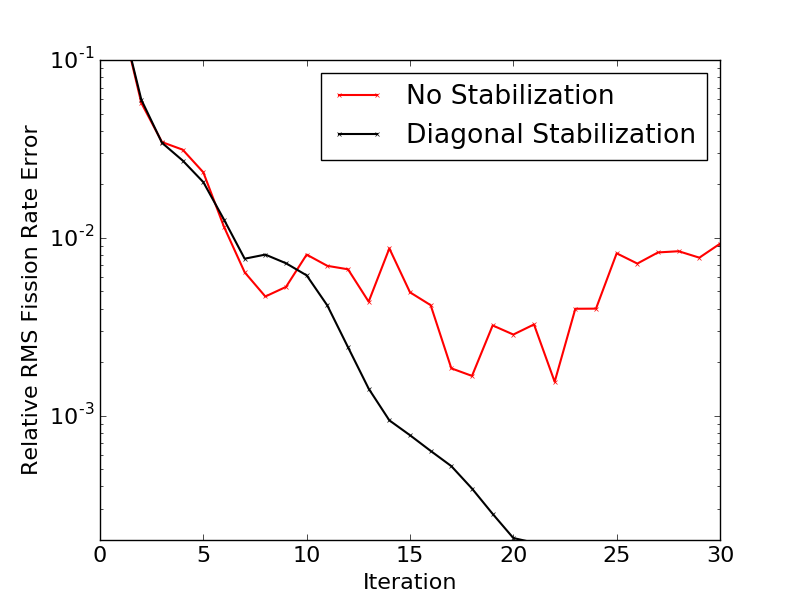
\includegraphics[width=0.71\linewidth]{figures/convergence/full-core-3D-ls.png}
	\caption{Convergence behavior of OpenMOC's linear source solver on the full core \ac{BEAVRS} benchmark with and without diagonal stabilization.}
	\label{fig:conc-fc-divergence}
\end{figure}

Results show that for reactor problems with large water reflector regions and a high number of energy groups, convergence of \ac{MOC} with reduced-group \ac{CMFD} acceleration is not possible without a stabilization scheme, such as diagonal stabilization. Full group \ac{CMFD}, in which the number of \ac{CMFD} groups match the number of \ac{MOC} groups, was always observed to converge. However, a reduced-group \ac{CMFD} acceleration scheme is often desired in order to reduce overhead.

It is important to note that this stabilization strategy has implications for all neutron transport solvers -- not just MOC solvers. Any solver which relies on source iteration has the potential to experience these same convergence issues when using transport-corrected cross-sections. Due to its wide-ranging applicability, this diagonal stabilization method is one of the most important contributions of this thesis to the reactor physics community. 

\subsection{Simulation Results}
\label{sec:sub:sim-results}

The OpenMOC 3D \ac{MOC} solver was used to simulate a variety of problems formed from the BEAVRS benchmark. Using the parameters necessary to reach spatial and angular parameter convergence, the full core BEAVRS benchmark was simulated.  The results are summarized in Table~\ref{tab:conc-table}, showing reasonable agreement with a reference continuous energy OpenMC Monte Carlo solution, from which the multi-group cross-sections were derived. 

\begin{table}[ht]
	\centering
	\caption{Simulation results of OpenMOC on the full core 3D BEAVRS benchmark using the Mira partition of the Argonne BlueGene/Q supercomputer compared with a reference OpenMC solution}
	\medskip
	\begin{tabular}{l|l}
		\hline
		OpenMOC $k_{\textit{eff}}$ &  0.99677\\
		OpenMC $k_{\textit{eff}}$ &  0.99927 +/- $1 \times 10^{-5}$\\
		OpenMOC RMS Fission Rate Error & 2.14\%\\
		OpenMC Avg. Fission Rate Std. Dev. & 1.82\% \\
		\hline
		OpenMOC Runtime & 7.76 hours \\
		CPU Cores & 92480 \\
		OpenMOC Computational Cost & 717,465 core-hours \\
		Estimated Computational Cost on Falcon & $\approx$ 200,000 core-hours \\
		\hline
	\end{tabular}
	\label{tab:conc-table}
\end{table}



%A slight tilt as observed from the center to the periphery of the core. This tilt is due to the particular transport correction that is not able to fully capture the effects of anisotropic scattering. It is possible that a better transport correction -- particularly in reflector regions -- would be able to eliminate this tilt.

Note that while the number of core-hours required to converge the problem is high (717,465), the solution was computed on the Argonne BlueGene/Q supercomputer, which has extremely slow cores for energy efficiency reasons. The requirements on modern computing cores, such as those on the Falcon supercomputer was estimated to be 200,000 core-hours.

To verify the chosen parameters were sufficient in converging the spatial and angular effects, a perturbation study was conducted on the full core, showing little sensitivity when parameters were refined. A recap of the axial \ac{MOC} parameters is given in Table~\ref{tab:conc-params}.

\begin{table}[ht]
	\centering
	\caption{Axial MOC ray and mesh parameters determined to accurately and efficiently simulate the BEAVRS benchmark}
	\medskip
	\begin{tabular}{lc}
		\hline
		Axial Ray Spacing & 0.75 cm \\
		Number of Polar Angles & 10 \\
		Axial Source Height & 2.0 cm \\
		\hline
	\end{tabular}
	\label{tab:conc-params}
\end{table}

This thesis was able to accomplish the full core simulation of an \ac{LWR} reactor, for the first time, using full core 3D deterministic neutron transport. These simulations can provide useful insight into the neutron behavior of rector geometries with complex geometric detail, such as the Westinghouse AP 1000\texttrademark. With this insight, safety margins could potentially be lowered, leading to more efficient and economic operation of modern nuclear reactors.

%%%%%%%%%%%%%%%%%%%%%%%%%%%%%%%%%%%%%%%%%%%%%%%%%%%%%%%%%%%%%%%%%%%%%%%%%%%%%%%%
\section{Future Work}
\label{sec:future-work}

\subsection{Accuracy Improvements of Full Core Simulations}

The \ac{MOC} solver developed in this thesis was able to reasonably simulate the BEAVRS benchmark. However, there was a noticeable tilt across the core due to the transport correction not properly accounting for anisotropic scattering. Therefore, this thesis illuminates the need for a better transport correction, particularly in reflector regions where the traditional flux-limited transport correction might not be sufficient. With an improved transport correction, the simulation results could be more accurate for the same computational cost.

\subsection{Further Full Core Analysis}

Future work in OpenMOC should also concentrate on reducing computational cost. Using the current solver, only uniform mesh refinement was studied for the axial direction in this thesis. A finer mesh could be used near reflector regions with a coarser mesh in the central core to improve accuracy and decrease computational cost. This would not require any further software development, only expanded analysis of full core reactor problems.

\subsection{OpenMOC Improvements}

Algorithmic implementation aspects of the OpenMOC could also be improved, including:

\begin{itemize}
	\item \textbf{Non-uniform Domain Decomposition}: The requirement of uniform spatial domain decomposition leads to load balancing inefficiencies, as observed on the BEAVRS benchmark. If domains could be merged, this issue might be alleviated.
	
	\item \textbf{Reduced Boundary Angular Flux Storage}: OpenMOC currently requires double storage of boundary angular fluxes so that information is not overwritten during their exchange between nodes. However, it might be possible to only store the information once if a clever algorithm is implemented to prevent overwriting of information. Since the memory usage is dominated by boundary angular flux storage, this would reduce the overall memory requirements by nearly a factor of two. Other approaches could also be examined where no boundary fluxes are explicitly stored, as implemented in APOLLO3~\cite{apollo3_exp} and ARRC~\cite{trrm_new}.
	
	\item \textbf{Non-uniform \ac{CMFD} Lattice}: Currently the OpenMOC \ac{CMFD} implementation requires uniform mesh for \ac{CMFD} acceleration. This is problematic for realistic full core problems where inter-assembly gaps exist. The inclusion of a uniform \ac{CMFD} lattice inserts extra discretization into the problem as \ac{CMFD} cell boundaries split \ac{MOC} source regions.
	
	\item \textbf{Splitting of \ac{CMFD} Cells Across Domain Boundaries}: Currently, domain boundaries cannot exist between \ac{CMFD} cells. This is not ideal for the BEAVRS benchmark in which assemblies contain a $17 \times 17$ lattice of pins. Since pin-cell \ac{CMFD} mesh is standard, this imposes limitations on how the assembly can be domain decomposed. 
	
	%\item \textbf{Inclusion of More General Linear Solvers for \ac{CMFD} Acceleration}: Currently, only a red-black SOR linear solver is available, which has a limited stability region. A more general linear solver, such as \ac{GMRES}, would allow for a fall-back if the red-black SOR linear solver fails to converge. 
	
	%\item \textbf{Improved Local Coordinates Structure}: The current coordinate data structure is not well designed. While it is only used for 2D ray tracing, which is not a significant computational cost, it could be greatly improved by changing from a linked-list representation to a vector representation.
	
	\item \textbf{Inclusion of a GPU Solver}: For 2D \ac{MOC}, Graphics Processing Units (GPUs) have shown the ability to solve \ac{MOC} equations efficiently. Similar results should be possible for 3D \ac{MOC}. 
\end{itemize}


\subsection{Spatial Source and Cross-section Approximations}

In addition to specific OpenMOC improvements, other 3D \ac{MOC} strategies could be introduced that have the potential for increased efficiency or accuracy using different spatial approximations.

First, different source approximations could also be studied in greater detail. Currently, a single source approximation (either flat or linear) is used for all regions in the core during a single simulation. However, within the modular framework, it is possible to create a solver which mixes flat and linear source approximations. For instance, moderator regions could always be simulated with a linear source approximation where there is a significant gradient, but gap and clad regions could be simulated with a flat source approximation where the neutron source is quite small. Additionally, source approximations restricted to only the axial direction, such as linear or quadratic, could be implemented for regions where radial variation is not significant.

In addition to implementing different source approximations, it would be useful to store spatial dependent cross-sections for depletion analysis.  In current methodologies, fuel is discretized into many regions in order to account for burnup gradients. If the variation could be captured with a spatially-dependent cross-section approximation, coarser mesh could allow for decreased computational cost of depletion studies.

\subsection{Treatment of Angular Dependence of Total Cross-sections}

It was noted in Appendix~\ref{sec:mgxs-angular-dependence}, the multi-group total cross-sections have an angular dependence and other authors have found a bias introduced by not accounting for the angular dependence~\cite{gibson-preprint}. Therefore, this should be treated in order to develop more accurate simulations capable of matching a fully converged continuous energy Monte Carlo solution. This could either be done by defining angular-dependent cross-sections, which could be computationally costly, or by correcting cross-sections through equivalence models~\cite{guillaume}.

\subsection{Convergence of Source Iteration with Linear Sources and CMFD Acceleration}

An important issue studied in this thesis was the convergence behavior of source iteration with transport-corrected cross-sections. However, the theoretical discussion of source iteration presented in this thesis relied on a flat source approximation without \ac{CMFD} acceleration. The diagonal stabilization scheme was shown to also work for \ac{CMFD} accelerated cases as well as the linear source solver, but a theoretical study would be useful, perhaps leading to an improved stabilization strategy.


\subsection{Reducing the Computational Requirements of Full Core Simulations}
	
Finally, the development of 3D transport methods should focus on making high fidelity reactor simulations even more efficient. The results presented in this thesis used many-group cross-section libraries and solution of the BEAVRS benchmark required a large supercomputer. These many-group cross-section libraries were used to reduce the spatial variation of cross-sections such that they are only dependent on the material, not the spatial location. However, \ac{LWR} simulations would be far more feasible if region-dependent several-group cross-sections were capable of accurately capturing neutron behavior. Therefore, future analysis should investigate several-group cross-section formations which maintain solution accuracy.